\chapter{Projektmanagement}

Im folgenden soll erläutert werden, wie diese Arbeit als Projekt organisiert und durchgeführt wurde. Dabei soll ein Überblick über die Projektstruktur sowie den Ablauf der einzelnen Arbeitsschritte gegeben werden sowie im speziellen auf die Implementierung der beschriebenen Lösungsansätze und Algorithmen eingegangen werden, da genau dieser Aspekt wohl klar die meiste Arbeitszeit in Anspruch nahm.

Es folgt eine übersichtsartige verbale Beschreibung der Arbeitsphasen und -schritte.

\section{Projektstruktur}

Um das Management während dem Projektverlauf zu erleichtern, wurde das Projekt in vier Teilbereiche, welche wiederum aus Arbeitspaketen bestehen, gegliedert, die in Gesamtheit alle Aufgaben, die im Rahmen des Projekts erledigt wurden, abdecken.

\begin{figure}
\centering
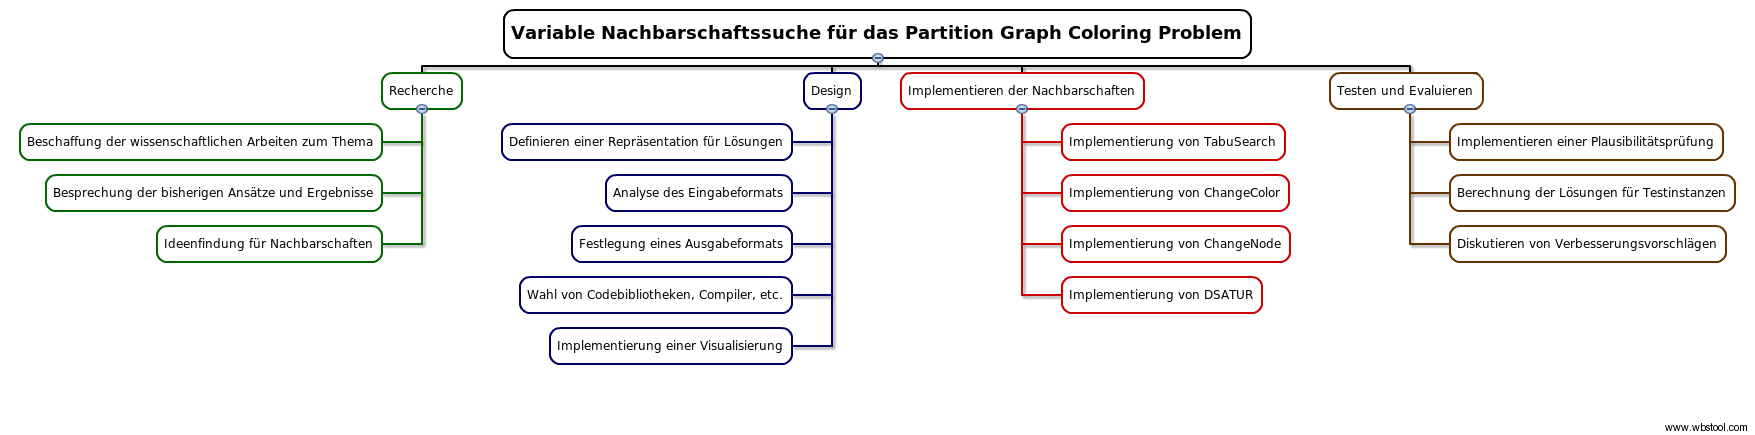
\includegraphics[angle=90, height=0.9\textheight]{img/psp.png}
\caption[Projektstrukturplan]{Pro\-jekt\-struk\-tur\-plan zur Übersicht über die Teilaufgaben innerhalb des Projektablaufs.}
\label{fig:psp}
\end{figure}

\subsection{Recherche}
Um nicht bereits zu Projektbeginn die Fehler anderer erneut zu begehen, erschien eine ausgedehnte Recherchephase sinnvoll. Rückblickend zeigte sich diese Phase als besonders hilfreich, um mit der komplexen Materie vertraut zu werden.

\subsubsection{Beschaffung der wissenschaftlichen Arbeiten zum Thema}

\begin{center}
\begin{tabular}{lll}
	Mitarbeit & Verantwortlichkeit & Betreuer informiert \\
	\hline
	Lorenz Leutgeb & Moritz Wanzenböck & ja \\
	Moritz Wanzenböck & & \\
\end{tabular}
\end{center}

Die wissenschaftliche Komponente des Projekts erforderte die umfangreiche Auseinandersetzung mit bereits abgeschlossenen Arbeiten zu ähnlichen Lösungsansätzen der gleichen Pro\-blem\-stel\-lung. Am wichtigsten hierbei ist das Identifizieren von wichtigen Erkenntnissen, die sich vorteilhaft für die eigene Arbeit nutzen lassen. So konnten wir beispielsweise schnell die Konstruktionsheuristik \textit{onestepCD} (siehe~\ref{sec:construct}) anderen Varianten vorziehen, da diese in früheren Evaluierungen die besten Ergebnisse berechnete.

\subsubsection{Besprechung der bisherigen Ansätze und Ergebnisse}

\begin{center}
\begin{tabular}{lll}
	Mitarbeit & Verantwortlichkeit & Betreuer informiert \\
	\hline
	Lorenz Leutgeb & Moritz Wanzenböck & ja \\
	Moritz Wanzenböck & & \\
\end{tabular}
\end{center}

Abgesehen von der Wahl von onestepCD aufgrund der offensichtlichen Vorteile wurde vor allem die Tabu-Suche von genauer analysiert, um daraus eventuell Schlüsse für leistungsfähige Nachbarschaften ziehen zu können. In der Tat führte dies zur Implementierung der Tabu-Suche als Nachbarschaft zu Testzwecken. %TODO referenz auf onestep, referenz auf tabusearch paper

\subsubsection{Ideenfindung für Nachbarschaften}

\begin{center}
\begin{tabular}{lll}
	Mitarbeit & Verantwortlichkeit & Betreuer informiert \\
	\hline
	Lorenz Leutgeb & Moritz Wanzenböck & ja \\
	Moritz Wanzenböck & & \\
\end{tabular}
\end{center}

Zum Abschluss der Recherchephase entwickelte sich bereits ein Gespür für die Struktur des Problems, sodass Ideen für eigene Nachbarschaften aufkamen. %TODO

\subsection{Design}
Nach einer Umfangreichen Recherche und Auseinandersetzung mit der Problemstellung ging das Projekt in die Designphase über. Hier galt es sicherzustellen, wie die Implementierung der Nachbarschaften erfolgen soll und außerdem Schnittstellen des Programms zur Außenwelt klar zu definieren.

\subsubsection{Definieren einer Repräsentation für Lösungen}

\begin{center}
\begin{tabular}{lll}
	Mitarbeit & Verantwortlichkeit & Betreuer informiert \\
	\hline
	Lorenz Leutgeb & Moritz Wanzenböck & nein \\
	Moritz Wanzenböck & & \\
\end{tabular}
\end{center}

\subsubsection{Analyse des Eingabeformats}

\begin{center}
\begin{tabular}{lll}
	Mitarbeit & Verantwortlichkeit & Betreuer informiert \\
	\hline
	Lorenz Leutgeb & Lorenz Leutgeb & nein \\
	Moritz Wanzenböck & & \\
\end{tabular}
\end{center}

Eine wichtige Eingabeschnittstelle des Programms ist das Einlesen von Probleminstanzen über die Standardeingabe. Hier wurde das Parsing zweier verschiedener Quellformate implementiert. Einerseits das \texttt{.pcp}-Format, in welchem ein Großteil der Instanzen vorlagen andererseits, das \texttt{.col}-Format.

\subsubsection{Festlegung des Ausgabeformats}

\begin{center}
\begin{tabular}{lll}
	Mitarbeit & Verantwortlichkeit & Betreuer informiert \\
	\hline
	Lorenz Leutgeb & Lorenz Leutgeb & nein \\
	Moritz Wanzenböck & & \\
\end{tabular}
\end{center}

Um die Ergebnisse der Berechnungen leicht auswerten zu können, wurde die Ausgabe aller Daten im JSON-Format beschlossen.

\subsubsection{Wahl von Codebibliotheken, Compiler, etc.}

\begin{center}
\begin{tabular}{lll}
	Mitarbeit & Verantwortlichkeit & Betreuer informiert \\
	\hline
	Lorenz Leutgeb & Moritz Wanzenböck & nein \\
	Moritz Wanzenböck & & \\
\end{tabular}
\end{center}

Bevor die Entwicklung des Programms tatsächlich beginnen konnte wurde eine Code\-bi\-bli\-othek gewählt, welche zusätzlich Zeit sparen und Fehlerquellen eindämmen sollte. Weitere Details siehe~\ref{sec:boost}

\subsubsection{Implementierung einer Visualisierung}

\begin{center}
\begin{tabular}{lll}
	Mitarbeit & Verantwortlichkeit & Betreuer informiert \\
	\hline
	Lorenz Leutgeb & Lorenz Leutgeb & ja \\
	Moritz Wanzenböck & & \\
\end{tabular}
\end{center}

Um die Arbeitsweise des Programms möglichst anschaulich darstellen zu können, wurde eine Visualisierung mit Ubigraph implementiert. Dies ermöglicht eine Überwachung der Ar\-beits\-schrit\-te einzelner Nachbarschaften, sodass auch Dritte Einsicht in den Ablauf gewinnen.

\subsection{Implementierung von Nachbarschaften}

\subsubsection{Implementierung von TabuSearch}

\begin{center}
\begin{tabular}{lll}
	Mitarbeit & Verantwortlichkeit & Betreuer informiert \\
	\hline
	Moritz Wanzenböck & Moritz Wanzenböck & nein \\
\end{tabular}
\end{center}

Als erstes wurde die Tabu-Suche implementiert, da eine ausführliche Beschreibung des Verfahrens vor lag. %TODO referenz tabusuche

\subsubsection{Implementierung von ChangeColor} %TODO moritz?

\begin{center}
\begin{tabular}{lll}
	Mitarbeit & Verantwortlichkeit & Betreuer informiert \\
	\hline
	Moritz Wanzenböck & Moritz Wanzenböck & nein \\
\end{tabular}
\end{center}

\subsubsection{Implementierung von ChangeNode} %TODO moritz?

\begin{center}
\begin{tabular}{lll}
	Mitarbeit & Verantwortlichkeit & Betreuer informiert \\
	\hline
	Moritz Wanzenböck & Moritz Wanzenböck & nein \\
\end{tabular}
\end{center}

\subsubsection{Implementierung von DSATUR}

\begin{center}
\begin{tabular}{lll}
	Mitarbeit & Verantwortlichkeit & Betreuer informiert \\
	\hline
	Lorenz Leutgeb & Lorenz Leutgeb & nein \\
\end{tabular}
\end{center}

\subsection{Testen und Evaluieren}

\subsubsection{Implementieren einer Plausibilitätsprüfung}

\begin{center}
\begin{tabular}{lll}
	Mitarbeit & Verantwortlichkeit & Betreuer informiert \\
	\hline
	Moritz Wanzenböck & Moritz Wanzenböck & nein \\
\end{tabular}
\end{center}

Um sicher zu gehen, dass die von den Heuristiken berechneten Lösungen plausibel sind, also keine Konflikte oder unerwünschte Verbindungen enthalten, müssen diese überprüft werden. Da dies mit steigender Instanzgröße nicht von Hand möglich ist, wurde ein simpler Plau\-si\-bi\-li\-täts\-check implementiert.

\subsubsection{Berechnung der Lösungen für Testinstanzen}

\begin{center}
\begin{tabular}{lll}
	Mitarbeit & Verantwortlichkeit & Betreuer informiert \\
	\hline
	Lorenz Leutgeb & Lorenz Leutgeb & ja \\
\end{tabular}
\end{center}

Um die Ergebnisse des in dieser Arbeit beschriebenen Ansatzes vergleichen zu können, wurden Testinstanzen herangezogen, welche als Richtwert dienen können.

\subsubsection{Diskutieren von Verbesserungsvorschlägen}

\begin{center}
\begin{tabular}{lll}
	Mitarbeit & Verantwortlichkeit & Betreuer informiert \\
	\hline
	Lorenz Leutgeb & Lorenz Leutgeb & ja \\
	Moritz Wanzenböck & & \\
\end{tabular}
\end{center}

Nach Abschluss des Projekts ist davon auszugehen, dass eine weitere Verbesserung der Ergebnisse möglich ist. In einer abschließenden Diskussion ging es darum, wie dieser Weg weiter verfolgt werden könnte.

\section{Risikoanalyse}
\begin{table}
\centering
\begin{tabular}{lccc}
Risiko & Eintreten $p$ & Ausmaß $s$ & Priorität $P$\\
\hline
Untergang der Welt mit Ende des 13.\ Baktun & $0.5$ & $1$ & $0.5$\\
Fehlende Vergleichsmöglichkeit der Ergebnisse & $0.25$ & $0.75$ & $0.1875$ \\
Fehlende Kenntnisse in C++ & $0.2$ & $0.8$ & $0.16$ \\
Datenverlust & $0.1$ & $0.9$ & $0.09$ \\
\end{tabular}
\caption{Übersicht über identifizierte Risiken}
\label{tab:risk}
\end{table}

Wie in Tabelle~\ref{tab:risk} ersichtlich ging von dem befürchteten Weltuntergang mit dem Beginn des nächsten \textit{Baktun}-Zyklus im Kalendersystem der Maya-Hochkultur eine große Gefahr für die Erfüllung der Projektziele aus, doch die präventive Verbarrikadierung des Projektteams am 21.12.2012 konnte  durchgehende Arbeit (zu diesem Zeitpunkt an der Implementierung) gewährleisten und erwies sich im Nachhinein als nicht zwingend nötig, da beim Verlassen des Hochsicherheitssystems am 22.12.\ keine dem Ereignis zuordenbaren größeren Infrastrukturschäden im Großraum Wien bemerkt wurden.

Das Absichern gegen weitere Risikoszenarien konnte aufgrund der weit höheren Priorität im Laufe der Vorbereitungen auf den Untergang der Welt nicht gewährleistet werden.

\section{Versionskontrolle}
Eine der ersten Entscheidungen im Laufe der Arbeit am Projekt, wahrscheinlich sogar schon vor der Wahl des Arbeitstitels, war die Auswahl eines geeigneten Versionskontrollsystems. Wie es die Teammitglieder für kleinere Projekte gewohnt waren, begann die Entwicklung in einem von einem Cloud Service bereitgestellten, synchronisierten Ordner. Doch schon nach wenigen Tagen war klar, dass eine für das Projektteam derart wichtige Arbeit ein voll ausgebautes und dezidiertes Versionskontrollsystem benötigt. Schnell fiel die Entscheidung auf \textit{Git}\footnote{\url{https://git-scm.org/}}, ein System, dass mitunter von den Entwicklern der größten Projekte der \textit{Free und/oder Open Source Software} eingesetzt wird.

Dabei beeindruckt Git vor allem durch den geringen Mehraufwand, um die Versionskontrolle zu pflegen. Weiters wurde es so möglich, komplett unabhängig an Dateien zu arbeiten und Änderungen im Nachhinein einfach zusammenzuführen.

\section{Continuous Integration}
Als zusätzliches Feedback-Element wurde in diesem Projekt auf Continuous Integration ge\-setzt. Das bedeutet, dass sobald Änderungen am Code in der Versionskontrolle eingecheckt und hochgeladen wurden, ein Webservice zur Verfügung stand, um die neue Version zu kompilieren und zu testen. Bei Fehlschlagen eines solchen Builds wurde das Projektteam instantan informiert, um möglichst rasch eine Fehlerbehebung zu beginnen.

Dies ermöglicht insbesondere auch die Überprüfung, ob der Code sich mit GCC genauso wie mit clang kompilieren lässt und bietet außerdem einen guten Richtwert der im Projektverlauf aufgetretenen Fehler. 
